\chapter{Preliminaries}\label{chapter:preliminaries}

\section{Cyber-Physical Systems}
\emph{Cyber-physical Systems} (CPS) are systems which are concerned with the coordinative interplay of computational and physical resources and processes. A CPS may be anything from a smart home application which allows users to unlock their doors via smart phone app, a collection of sensors dispersed in an industrial plant that report on a product's quality attributes, to a smart grid that algorithmically controls a region's electricity production and distribution.
%an air-conditioning system which automatically turns off once the apartment's residents have left the house.
%or an autonomously driving vehicle which relies on cameras and lidars to navigate through traffic.
All these examples have in common that they involve physical, tangible appliances which are tightly intertwined with computing systems.
CPS retrieve information about the physical world through sensors, bring the sensed data into machine readable form, process it and act upon it to exert influence on their environment. More often than not, CPS occur as collections of dispersed components which are connected not only to each other, but also to the Internet. Thus, a CPS' perception is not limited to its own physical locality, but it can also make use of globally available data and services \cite{broy2012cyber}. In this context, the term \emph{Internet of Things} (IoT) is commonly used to describe connected amalgamations of computing devices that exist ubiquitously in the environment.

%\paragraph{Automotive System Engineering}
The one type of CPS that this thesis is mostly concerned with are vehicles. Modern vehicles perceive the environment through a variety of sensors (\eg\ cameras, lidars,\footnote{``LIght Detection And Ranging''} short and long-range radars, etc.), and use that information to make informed, autonomous decisions to ensure the continuous operability of the vehicle and to implement comfort functions.  
Beyond the immediate, physical awareness (distance, velocity, location, etc.) that is needed to make such decisions, the CPS needs to deduce situational awareness (\emph{how is the information relevant to the current situation?}) as well as contextual awareness (\emph{which other factors may influence the decision?}). 
The evolution of vehicular braking systems is an example of a traditional, mechanically driven subsystem that, with time, turned into a sophisticated, algorithmically controlled ``system of systems'' which considers more factors than just the brake pedal's position. This example is lent from the remarks of \citeauthor*{broy2012cyber} \cite{broy2012cyber}.
In the late seventies, the Anti-lock Braking System (ABS) was developed as a simple mechanism to ensure maneuverability of the vehicle while braking. It functions rather primitively: if a sensor detects that a wheel rotates too slowly, compared to the vehicle's speed (indicating a wheel lock), valves are actuated to reduce the brake's hydraulic pressure, effectively causing a reduction in braking power to ensure the wheel's traction needed for steering. This process, in its simplest form, is a purely mechanical reaction to sensor input.
This is in contrast to modern braking systems which, in addition, take situational factors into consideration. For instance, Electronic Stability Control (ESC) monitors the state of the vehicle and compares that to the state that the vehicle \emph{should} be in, according to the driver. For this, the system considers, \eg , the position of the steering wheel and thus deduces the driver's intent to maneuver the vehicle in another direction. If the vehicle's actual condition and the desired condition deviate by a too large degree, the ESC takes measures. More advanced braking systems, such as Active Brake Assist (ABA), additionally rely on cameras to detect obstacles in front of the vehicle, present a warning to the driver if danger is imminent, and, if required, brakes autonomously.
The evolution of vehicular braking systems exemplifies the gradual progression from isolated, single-purpose functions to complex CPS which make decisions based on contextual information inferred from sensor data from a multitude of different subsystems. Likewise, similar evolutions can be observed in many other parts of our everyday life as ordinary ``things'' become connected and computing becomes pervasive.

%Control systems in modern vehicles are typically implemented as a collection of dozens, if not hundreds, of Electronic Control Units (ECUs) dispersed within a vehicle. Originally, there was no conscious decision to design automotive systems that way. Much rather, it is the result of an evolutionary process. At first, individual ECUs, each dedicated to a single purpose, were implemented in vehicles. At this point, ECUs were isolated from each other and no sense of cohesion was present in the system. This changed with the introduction of advanced wiring and bus systems that allowed ECUs to interact with sensors and actuators. It was then only a matter of time until the bus systems were used to furthermore interconnect ECUs, which could then be used in interplay to create new, innovative functions \cite{broy2006challenges}.
%However random this evolution might have been, there are several benefits to the dispersed approach (as opposed to a centralized one). By having ECUs close to the sensors and actuators they control, wiring effort is kept low, which results in low transmission latencies.

%Problems according to \citeauthor*{broy2006challenges}:
%\begin{itemize}
%\item Often highly proprietary
%\item Limited re usability of software: 90\% of software is re-written
%\item Lack of tools and automation
%\end{itemize}


%Industry profile according to \citeauthor*{broy2006challenges}:
%\begin{itemize}
%\item Highly modular: several teams working independently on different technologies
%\item Much is outsourced: many technologies are developed by suppliers, rather than the OEM
%\item Development: Many systems must interact -> vehicles evolve from an assembled device to an integrated system
%\item Behavior becomes programmable: from comfort functions to steering and breaking: everything can be controlled by software.
%\item moving away from specialized ECUs to general-purpose commodity systems
%\end{itemize}

%
%
%
%
%
%
%
%
%
%

\section{Distributed Systems}
Modern vehicular E/E-architectures\footnote{``Electric/Electronic architectures''} are comprised of a large number of distributed, connected sensors, actuators and Electronic Control Units (ECUs) \cite{navet2005trends}, and hence, fall into the category of \emph{distributed systems} \cite{leen2002expanding}. The term ``distributed system'' entails many things and just as many definitions of the term exist. A definition that most would agree upon is the one given by \citeauthor{tanenbaum2017distributed} \cite{tanenbaum2017distributed}:
\begin{quote}
``A distributed system is a collection of autonomous computing elements that appears to its users as a single coherent system.''
\end{quote}
The first aspect to consider in this definition is the word \emph{collection}. Distributed systems are made up of a number of \emph{nodes} which may occur in the form of either hardware devices, or software processes. Nodes work together to achieve a common goal. For this, they need to exchange messages. More on the communication aspect is discussed in \Cref{sec:middlewares}. Furthermore, the definition names \emph{autonomy} as a characteristic of distributed systems. Nodes, on their own, are autonomously acting entities, with their own, individual sets of rules and behavior. At the same time the system needs to be kept together. \emph{Groups}, which individual nodes may join, are a tool to achieve this. There are open groups, which every node may join, and closed groups, which employ an authorization mechanism to control access.
Groups aim to provide \emph{coherence}, which is another aspect of the definition given above. By the given definition, however, the coherence of the system is only \emph{perceived}. \Ie , to users, whether they are humans or programs, a distributed system presents itself as a single entity, even though it is in actuality comprised of a number of physically dispersed processes and resources. This principle is called \emph{distribution transparency}. \citeauthor*{tanenbaum2017distributed} \cite{tanenbaum2017distributed} separate this principle into several aspects. The first one to note is \textbf{location transparency}. At the root of location transparency is the desire to hide the physical location of resources. A common method to achieve this is through the assignment of names. A user who wants to access a resource can thus refer to it by name, \eg\ a URL,\footnote{``Uniform Resource Locator''} while remaining oblivious of its actual location. Under the hood, communication is still based on location-dependent addresses, but such details can be hidden by a name resolution service.
Naming furthermore facilitates another kind of distribution transparency: \textbf{Relocation transparency}. As the name suggests, relocation transparency aims to hide the fact that resources may move from one location another without the user taking notice. In the example of the aforementioned name resolution service, this can be achieved by reconfiguring the service to redirect users to a location different than the one previously known. To the user, still, the resource appears to be in the same location as it only knows its name.
Related to relocation transparency is \textbf{migration transparency}, but in contrast to the former, migration transparency refers to the mobility of the \emph{user}. A migration transparent system allows a user to roam freely, while maintaining connectivity to the rest of the system. Examples of such systems are cellular networks.

Another aspect of distribution transparency is \textbf{replication transparency}. Distributed systems often provide means to replicate nodes or resources, \eg\ to improve availability and scalability. Replication transparency states that all such replicas appear as one to the user. In addition to scalability, replication can be helpful to provide failure resilience. If a given node fails, and a replica is available, the user can be automatically redirected to the replica. This is also known as \textbf{failure transparency}.

Another way in which a distributed system can be transparent is in terms of concurrency. Resources are often times shared among a number of users which are concurrently using the system. A desirable trait thereby is to hide this fact from the user such that the they are lead to believe that they are the only one with access to that resource. This is called \textbf{concurrency transparency}.

%The last kind of distribution transparency that \citeauthor*{tanenbaum2017distributed} define is \textbf{access transparency}. Access transparency refers to how data is presented to different users. Several users may have entirely different views of the same data\todo{explain better}. At the basis of this is a basic principle of software engineering: the separation of data and its representation.

%
%
%
%
%
%
%
%
%
%

\section{Middlewares} \label{sec:middlewares}
A prerequisite for the coherence property of distributed systems is the need for nodes to engage in collaboration. More precisely, distributed applications need a way to pass messages, or data, between different threads of execution. For this purpose, \emph{middlewares} \cite{bernstein1996middleware} are commonly used. Although message passing is a prime example of a middleware's use case, there are many other important concepts for which middlewares exist, \eg , transaction management in database systems. The primary goal of middlewares is to abstract away complex concepts so that programmers can focus on implementing business logic and shipping features, instead of having to deal with the underlying specifics. Middlewares are implemented as a software layer that sits between operating system and the actual applications. They are often included in the form of libraries that make the middleware's functionality available to the programmers by means of an Application Programming Interface (API).

The need for middlewares becomes particularly evident in the example of messaging. Messages need to be sent over a physical mediums which are often, by nature, unreliable. To ensure reliability, many things need to be taken care of, \eg , error detection, repetition mechanisms, etc. In addition, guarantees must be given that messages are delivered to the right receivers. Therefore, addressing and routing mechanisms must be in place. Thes
e are just a few examples of hard-to-solve problems related to messaging. Managing these things manually, and implementing according measures from the ground up is hardly feasible for programmers. Messaging middlewares greatly simplify this process.

\begin{lstlisting}[caption={[Middleware send example]A code snippet demonstrating a broadcast dispatch via middleware}, label={lst:send}, language={C++}]
auto& middleware = MW::register_by_name("Alice");
middleware.broadcast("Hello, World!");
\end{lstlisting}

\begin{lstlisting}[caption={[Middleware receive example]An exemplary callback function to receive messages via middleware}, label={lst:receive}, language={C++}]
void receive(const std::string& message, const std::string& sender)
{
  // message = "Hello, World!"
  // sender = "Alice"
}
\end{lstlisting}

\Cref{lst:send} and \Cref{lst:receive} show code snippets demonstrating the sending and receiving capabilities of a hypothetical messaging middleware. In the example, all a programmer needs to do to send messages is to invoke a simple function, \eg , \texttt{sendBroadcast} in \Cref{lst:send}. The middleware then ensures that the message is delivered to the right recipients over whichever transport is available. To receive messages, the programmer may, in the case of this exemplary middleware, define a callback function which the middleware calls automatically whenever a new message is available. An example of such function is depicted in \Cref{lst:receive}. In the callback function's body, logic could be implemented to process the message content passed in the \texttt{message} parameter.

%
%
%
%
%
%
%
%
%
%

\section{Cloud Computing}

The idea of cloud computing is to provide access to remote computing resources  (\eg , networks, servers, storage, applications, and services) in a convenient, on-demand manner \cite{mell2011nist}. Customers of cloud providers can rent these resources to use them at their will. By outsourcing their IT infrastructure into the cloud, companies can significantly reduce capital and operational expenditures (CAPEX/OPEX) that are typically associated with running an on-premise infrastructure\todo{citation}. Other benefits include easier maintenance and accelerated time-to-market times\todo{citation, mehr benefits?}. Several pricing models for cloud services exist. Customers often have the choice between a set monthly fee, or they may take advantage of a pay-per-use model, whereby providers bill their users, \eg , on the basis of CPU time.

Cloud infrastructures are typically implemented as multi-tenancy systems in which the same hardware is shared among many customers. This principle is known as ``resource pooling''. An enabling technology for this is virtualization. Each customer is assigned one or more virtual machines (VMs) running on one or more physical servers. For its users, the alloted computing environment appears as a single, isolated physical machine. The amount of disposable resources can be controlled for each VM individually, allowing for fine-grained resource tuning according to demand.

A major selling point of cloud computing is scalability. Many cloud providers allow for the dynamic allocation of resources depending on demand. To customers, the available resources appear as if they were unlimited when in actuality the substrate resources are alloted and released under the hood in an elastic manner. To steer this behavior, \emph{elasticity controllers} can be employed which allow customers to define rules to control when and how scaling measures are performed. \Eg , when a CPU utilization threshold is reached, the system can be instructed to automatically launch an application replica. Subsequently, a load balancer can be used to distribute the load between the instances \cite{vaquero2011dynamically}.


\paragraph{}
Cloud computing occurs in the form of several usage models. The most notable ones are: \emph{Infrastructure as a Service} (IaaS),  \emph{Platform as a Service} (PaaS), and \emph{Software as a Service} (SaaS) \cite{mell2011nist}, but many other models, mostly derivatives of the three mentioned, are in use today.

\begin{description}
\item[IaaS] In the IaaS model, sheer, usually virtualized, hardware is provided, on which customers can install and run arbitrary software. Customers have only basic control over their virtual infrastructure's hardware composition, but may exert influence on the operating system level.
\item[PaaS] The PaaS model presents a higher level view on the infrastructure. In this model, customers don't have full control over their VM instance. Instead, they can deploy their software in predefined application-hosting environments \cite{mell2011nist} which are typically centered around a certain technology, \eg\ .NET, Node.js, etc. Examples for this type of services are Microsoft Azure or Google App Engine.
\item[SaaS] Finally, at the highest abstraction level of cloud usage models is the SaaS model\todo{sounds weird}. SaaS typically describes applications which are hosted on cloud platforms. These applications are usually accessible by means of thin clients, and most notably web browsers. Customers have the least control over the cloud service and can only exert influence via application-level configurations \cite{mell2011nist}. Examples of SaaS applications are browser-based e-mail services or video streaming platforms.
\end{description}

%
%
%
%
%
%
%
%
%
%

\section{Overlay Networks} \label{sec:overlays}
Distributed systems are often organized as \emph{overlay networks}\footnote{The term ``overlay networks'' is often used interchangeably with its abbreviated form, ``overlays''} \cite{tarkoma2010overlay}. An overlay network is a logical network which connects nodes, or peers, in an abstract, high-level manner. Naturally, in order to enable information exchange between the peers, overlay networks require a substrate physical network (\emph{underlay}) over which data can be transmitted. As opposed to physical networks, which connect \emph{physical machines}, overlay networks connect \emph{processes}. An important thing to note is that overlays aim to be as decoupled as possible from their respective underlays, such that both networks may evolve (change topology) independently without affecting their operability \cite{tanenbaum2017distributed}. For example, an added node in an overlay network does not necessarily entail the addition of a physical node. Conversely, the removal of a physical node does not necessarily result in connection loss of a logical node. An example of this is the Internet \cite{vaezi2017virtualization}, which spans a worldwide network of nodes that is resilient to failures, such that, when a physical node breaks, a redundant path to the target node may be taken. Other examples of overlay networks are VPNs, Peer-to-peer (P2P) networks and voice over IP (VoIP) systems. A schematic example of an overlay network is depicted in \Cref{fig:overlay}. The overlay spans over an underlay network, which in turn consists of three sub-networks. These sub-networks could be, \eg , company's internal network, the Internet, and a network within a data center.

\begin{figure}[htpb]
  \centering
  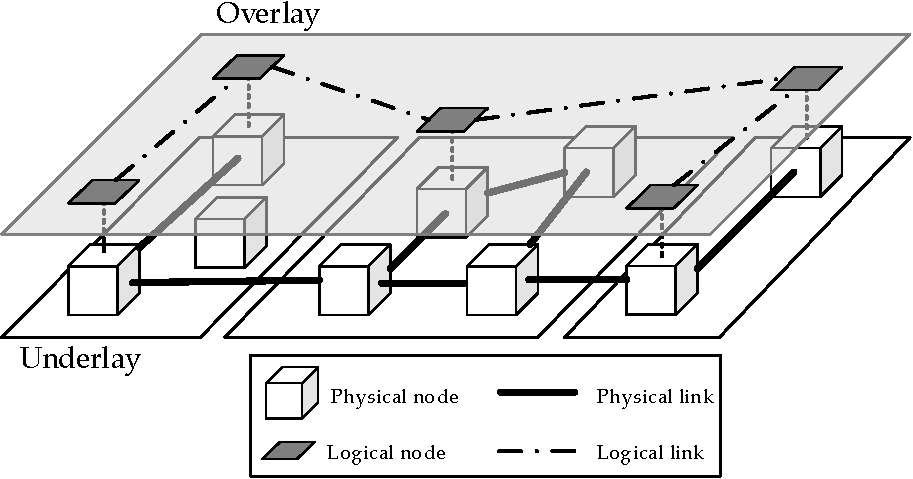
\includegraphics[width=0.8\textwidth]{figures/overlay.pdf}
  \caption[Overlay networking concept]{An overlay network on top of a physical underlay network which consists of three sub-networks}\label{fig:overlay}
\end{figure}

A distinction between two types of overlay networks is made: \emph{structured} and \emph{unstructured} ones. In the former, peers are organized in a specific, deterministic manner, such that each node has its firm place and an immutable set of neighbors. Unstructured overlay networks, on the other hand, allow the topology to change dynamically. In order for this to work, each node maintains an ad-hoc list of neighbors that is to be updated continuously \cite{tanenbaum2017distributed}. In the context of this thesis, unstructured overlay networks are of particular interest due to the dynamic nature and the reliability characteristics of mobile systems.

\paragraph{Virtual Local Area Networks.}
There are a number of ways to realize logical network overlays. VXLAN\footnote{``Virtual eXtensible Local Area Network''} and NVGRE\footnote{``Network Virtualization using Generic Routing Encapsulation''} two common examples which implement overlays on network datagram level. The technology used in the context of this work builds on VXLAN \cite{rfc7348}, an encapsulation protocol based on the long-established Virtual LAN (VLAN). VLANs make it possible to segregate a physical network into several isolated, logical networks. Each of those logical networks is assigned an identifier, a so-called \emph{VLAN tag}. All packets sent within a VLAN network have their respective network's VLAN tag attached on them at data link level (layer 2 in the OSI\footnote{``Open Systems Interconnect''} model). Based on the packet's tag, the substrate infrastructure can make decisions on how, and where, to forward packets. This allows for the realization of broadcast domains: each broadcast originating from a given VLAN network will stay within that network, regardless of how many other virtual networks exist alongside. This helps to significantly reduce network traffic.

Since the time when VLAN was devised much in the technological landscape has changed. In particular, virtualization has made great strides with the advent of cloud computing and multi-tenancy systems. Nowadays, thousands of virtual nodes dispersed throughout different clouds and on-premise infrastructures need to be connected. With its limited support for only 4096 virtual networks, VLAN cannot meet these increased demands. Thus, VXLAN was devised as a way to deal with the changed requirements.
The most notable changes, compared to VLAN, is the support for up to 16 million virtual networks and the option to assign addresses to \emph{processes}, rather than \emph{devices}.
In contrast to VLAN, which is an intrinsic part of layer 2 protocol frames, VXLAN is an independent protocol which is placed on top of UDP connections (in the application layer). This is illustrated \Cref{fig:vxlan} in which the VXLAN protocol stack is depicted. VXLAN works by wrapping the original data packet sent from one application to the other in a VXLAN frame which is then placed inside a UDP frame. As a result of this, two sets of addresses exist: the logical (source and destination) MAC addresses embedded in the encapsulated packet, and the physical MAC addresses in the surrounding packet.
Consequently, two types of packet switching need to be performed: once on a logical level, and once on a physical level. While physical switching is still performed inside physical network switches, an additional, logical type of switching needs to be introduced. Open vSwitch \cite{pfaff2015design} is an example of a virtual, software-based switch that performs packet switching in the data plane (within the Linux kernel).

\begin{figure}[htpb]
  \centering
  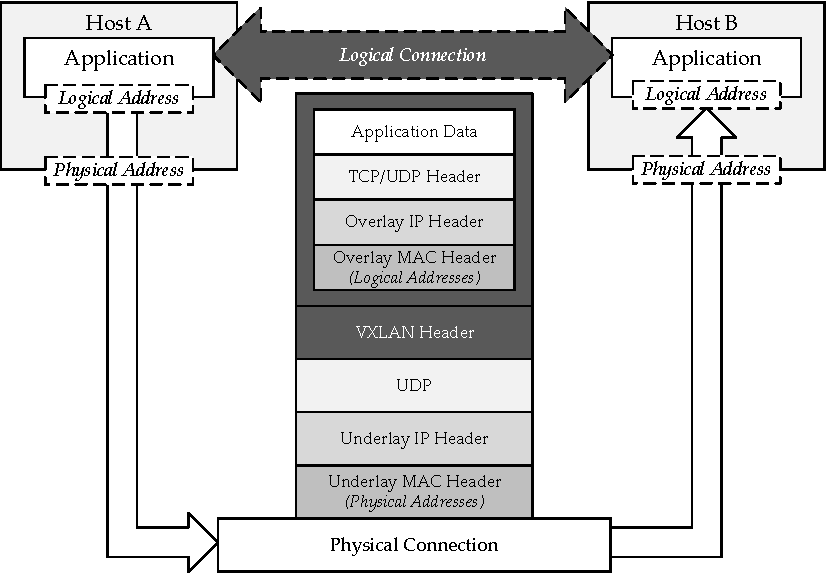
\includegraphics[width=0.9\textwidth]{figures/vxlan.pdf}
  \caption[VXLAN protocol stack]{VXLAN protocol stack exemplified by two logically connected applications}\label{fig:vxlan}
\end{figure}

Since VXLAN utilizes virtual MAC addresses that don't necessarily need to correspond to actual hardware addresses, addresses can be assigned at will for each process or virtual machine. This makes it possible to address single VM instances within an overlay network individually, regardless of physical locality and the underlying network design. An added benefit is that all endpoints may retain their logical address when migrating to other physical nodes. This allows for the creation of dynamically changing networks in which processes may move between different execution environments. Furthermore, VXLAN addresses the problem that WANs, in general, lack support for point-to-multipoint communication. In the context of an overlay network, peers may send messages to several receivers simultaneously, \eg\ by means of IP multicast, regardless of their physical location.
%Also included in the VXLAN header is a 24-bit network identifier which allows for the creation of 16 million virtual overlay networks, which is a tremendous step up from classic VLAN.

In essence, VXLAN is a layer 2 overlay scheme on layer 3 networks which effectively creates \emph{tunnels} between Virtual Tunnel Endpoints (VTEPs), indicated by the dashed ``Logical Address'' boxes in \Cref{fig:vxlan}. Thus, logical connections in VXLAN overlays are often referred to as ``VXLAN tunnels''.
%Encapsulated within each VXLAN frame is the actual packet sent from one application to another. Addressing in VXLAN is based on MAC\footnote{``Media Access Control''} addresses.


%\subsection{Multicast}
%The simplest form of communication is one-to-one communication, which is also referred to as \emph{unicast}. In unicast, every node has an address by which it can be contacted. In most cases, unicast is sufficient for data exchange. However, in distributed systems, information frequently needs to be propagated to multiple receivers simultaneously. Unsurprisingly, this type of communication is called \emph{multicast} communication.

%benefits: No hard-coded addresses

%Multicast can be implemented on both, network and application-level.

%Support for multicast in WANs is rather limited.

\pagebreak
\section{Containerization}
In recent years, container technology has gained widespread adoption in the software development world. By providing light-weight, portable execution environments for applications, containers greatly simplify the software development and deployment workflow, and thus have become a cornerstone of modern software architectures.

\subsection{Comparison to Virtual Machines}
Containerization is also known as ``operating-system-level virtualization'' \cite{soltesz2007container}, and thereby disassociates itself from traditional virtualization technologies such as virtual machines. A major difference between the two is that containerization does not rely on an intermediate virtualization layer between application and hardware, whereas VMs employ hypervisors for this purpose. Hypervisors make it possible to run entire operating systems in their own, isolated environments, so-called VM instances. Several instances may run on the same host machine side-by-side without affecting one another, which allows for the realization of multi-tenant systems. Since hypervisors abstract the substrate hardware, a layer of indirection between hardware and the application to be executed is added. The consequence of this is a considerable overhead, compared to native execution. Containers, in contrast, run directly on the host's kernel and thus exhibit near-native performance (\cite{adufu2015container, felter2015updated, morabito2015hypervisors}). This approach, however, bears security issues~\cite{xavier2013performance}.

As mentioned, each VM instance contains its own operating system and kernel. As a consequence, the disk space requirements for VMs are comparatively high. Additionally, the guest OS within a VM needs to be booted into before being operational, which slows down the VM's start-up speed. Containers, in contrast, do not include their own OSes and kernels. Thus, container start-up can be performed in a matter of milliseconds and is more akin to spawning a process, rather than booting an OS. This enables them to be created and destroyed depending on situational demand, which allows for the implementation of highly elastically scaling systems.
%The recently emerged Function as a Service (FaaS) paradigm popularized by Amazon's cloud offering, AWS Lambda\footnote{\url{aws.amazon.com/de/lambda}}, even suggests to run an ephemeral container for each \emph{request}
Considering their advantages over hypervisor-based virtualization, such near-native performance, sub-second boot times, minimal disk space usage and their energy efficiency \cite{morabito2015power}, containers bring qualities to the table that are relevant especially to embedded systems, which are, by their very nature, resource-constrained. Unsurprisingly, the possibility of leveraging containerization in embedded environments has received substantial attention in recent years (\eg\  \cite{bellavista2017feasibility, javed2016container, morabito2017virtualization}).

Containerization and virtual machines are often regarded as competing virtualization technologies. However, both are not mutually exclusive. In fact, most IaaS providers base their infrastructure on traditional VMs, which then, in turn, host container runtimes~\cite{dua2014virtualization}. Containers and VMs shall thus be seen as complementary, rather than competing, technologies.

\subsection{Container Internals}
Like virtual machines, containers aim to isolate processes from their environment. In the case of containers, isolation is achieved by a kernel feature called \emph{kernel namespaces}.\footnote{\url{www.man7.org/linux/man-pages/man7/namespaces.7.html}} Namespaces wrap global system resources, such as network devices and mount points, and present them to processes as if they were dedicated to them.
When a process runs in the context of a certain namespace, its access and view is limited to that namespace.
There are seven types of namespaces, each of which isolates a different aspect of the host system.
An example for this are \emph{process} namespaces which allow for the creation of alternative views on the process tree. For instance, consider a hypothetical process with PID 345. By assigning a process namespace to that process, it can be led to believe that it has the PID 1 and is the only process running on the system. Thus, the processes' view on other processes is restricted, and since a process can only access what it can see, isolation is achieved.
In a similar way, a processes' access to networks interfaces, the file system, user groups and other parts of the host system can be restricted.

In addition to providing isolation, containers employ resource management mechanisms which make it possible to allocate and limit the resources available to them. Resource management for containers is implemented by a kernel feature called \emph{control groups}, or \emph{cgroups}\footnote{\url{www.man7.org/linux/man-pages/man7/cgroups.7.html}} in short. Cgroups allow for the organization of processes in hierarchical groups. On these groups, resource constraints can be imposed (\eg\ CPU-time, access to devices, memory budget, etc.).
Through this mechanism, processes can be bundled together, effectively forming \emph{containerized process trees}, which can be restricted in what they can do and which resources they may take up. This opens up the possibility for container engines to exert fine-grained control over each processes' resource utilization and to further isolate processes from the rest of the system.

The two concepts (namespaces and cgroups) can be applied individually to any given process running on a Linux system. Only when combined together, such that processes are isolated through namespaces and restricted through cgroups, we speak of containers. In consideration of this, it becomes clear that a containerized process is not much different from a regular process. Rather, containers should be viewed as processes which are \emph{augmented} by these two concepts.

%Further separation can be achieved through SELinux and AppArmor.

While it is possible to create containers manually utilizing the aforementioned native kernel features, such undertaking is rather cumbersome. For this reason, several tools are being developed which aim to streamline the use of containers. A few notable examples are \emph{\docker},\footnote{\url{www.docker.com}} \emph{RKT},\footnote{\url{www.github.com/rkt/rkt}} \emph{CRI-O},\footnote{\url{www.cri-o.io}} \emph{Railcar}\footnote{\url{www.github.com/oracle/railcar}} and \emph{LXC}.\footnote{\url{www.linuxcontainers.org}} Among these,  \docker\ is undoubtedly the most prominent one, and arguably the first one to make Linux containers accessible for general use. As it is the most mature containerization solution, \docker\ was chosen for the approach presented in this thesis.







%
%
%
%
%
%
%
%
%
%

%\section{Software Architectures}
%\todo[inline]{
%Today, there is a tendency for software architectures to shift away from the \emph{monolithic} paradigm of having a single software entity deployed on a single, potent server to a more \emph{distributed} paradigm where multiple components are spread over a number of less potent physical hosts connected over a network.
%The benefits of this approach became evident in the early 2000's when a new type of software architecture utilizing this concept became popular: \emph{service-oriented architectures} (SOAs).

%In recent years, SOAs have made a revival in the form of \emph{microservices}, which, in essence, is a more fine grained type of SOA that avoids the complexity induced by \emph{Enterprise-Service-Buses} (ESBs). Similar to SOA, the idea behind microservices is to split functionality into a collection of reusable components, each fulfilling a single specific purpose. Recent research efforts are evaluating the possibility to include such paradigm in the realm of automotive software systems -- in part achieving great success \cite{berger2017containerized}.

%Since Microservices are very limited in scope they may be built and deployed in a matter of minutes, rather than hours, as is the case with monolithic applications. Thus, microservices have the potential to tremendously accelerate the software development process when being combined with modern development practices such as \emph{continuous integration / continous delivery} (CI/CD).
%}
